\section{Background and Motivation} \label{sec:background}
As per the title, in this paper we present a case for the necessity of understanding assurances, and in doing so also present a definition. Finally we perform a survey of methods by which assurances have been calculated.

Motivations and a grounding application are presented in Sections~\ref{sec:motivation} and \ref{sec:mot_example}, along with some application-specific definitions of the trust-cycle terms. A discussion of related work is in Section~\ref{sec:rel_work}. Section~\ref{sec:aias} defines the term AIA in a general sense, and highlights how they relate to assurances. Section~\ref{sec:trust} discusses trust, and provides a model of human-AIA trust that can be used in designing assurances. Section~\ref{sec:trbs} discusses trust-related behaviors and how they should be considered when designing assurances. Finally, a preliminary, simple, definition of assurances is presented Section~\ref{sec:assurances}. 

\subsection{Motivation} \label{sec:motivation}
    What do people who talk about `comprehensible systems', `interpretable learning', `opaque systems', and `explainable AI' really, fundamentally, care about? Generally, humans want to trust \footnote{Of course, at this point `trust' is quite an imprecise term, and will be defined more formally in Section~\ref{sec:trust}} the tools and systems that they create. To this end many metrics and methods have been created to help assure the designers and users that the tools and systems are, in fact, capable of being applied in certain ways, and/or will behave as expected. 

    The situation has grown more complicated in recent years because the advanced capabilities of the systems being created can at times be difficult, for even those who designed them, to comprehend and predict. There are, for instance, systems that have been designed to learn from extremely large amounts of data, and are expected to regularly perform on never before seen data. In some cases, such systems have been designed to perform tasks that might take humans entire lifetimes to complete. Below is a sample of some application areas and possible reasons why they have an interest in creating trustworthy systems:

    \begin{description}
        \item [Artificial Intelligence/Machine Learning:] There is a need to interpret how and why theoretical AIA models function, in order to know they are being applied correctly and to design new approaches to overcome weaknesses in the existing methods~\cite{Garcia2015-rs,Otte2013-oo}.    
        \item [Interpretable Science:] Scientists need to be able to trust the models created using data analysis, and be able to draw insights from them. Scientific discoveries cannot depend on methods that are not understood~\cite{Faghmous2014-og}.
        \item [Reliable Machine Learning:] It is critical to have safety guarantees for AIAs that have been deployed in the real world. Failing to do so can result in serious accidents that cause loss of life, or significant damage~\cite{Sugiyama2013-ci,Amodei2016-xi}.       
        \item [Public Policy:] Governments are beginning to enforce regulations on the interpretability of certain algorithms in order to ensure that citizens can understand why AIA driven services make the decisions and predictions that they do. A specific example are the algorithms deployed by credit agencies to approve/reject loans~\cite{Wagner2016-ck}.
        \item [Medicine:] Medical professionals need to understand why data-driven models give predictions so that they can choose whether or not to follow the recommendations. While AIAs can be a very useful tool, ultimately doctors are liable for the decisions they make and treatments they administer~\cite{Jovanovic2016-gw}.
        \item [Cognitive Assistance:] Systems are being designed as aids for humans to make complex decisions, e.g. searching and assimilating information from databases of legal proceedings. When an AIA presents perspectives and conclusions as data summaries, it must be able to also present justifying evidence and logic~\cite{Gutfreund2016-xe}.
    \end{description}

    The interests of the author lie specifically in the design of unmanned vehicles that operate in concert with human operators in uncertain environments. In this setting, it is desirable for unmanned vehicles to communicate with operators in some way to help them properly interact with the vehicle. The hope is that, in doing so, the performance of the team can be improved by appropriately utilizing the strengths of both the human and unmanned vehicle. This application is explained in more detail below in relation to Figure~\ref{fig:SimpleTrust_one_way}.

    \brettcomm{Important---Whether formally acknowledged or not, human AIA system designers and users want \emph{assurances} to help them appropriately trust AIAs. There are a few research fields that have formally and explicitly considered trust between humans and technology, e.g. e-commerce, automation, and human-robot interaction. However, these research efforts have mainly focused on implicit properties of the systems that affect trust. Conversely, there are other fields that have informally considered how to affect the trust of designers and users via explicitly designed assurances. However, due to their informal treatment of trust, it is unknown and unclear how effective these designed assurances might be in practice, or what principles ought to be considered when designing assurances for general AIAs. The goal of this paper is to survey these areas and, in doing so, help bridge the gap between them by identifying common goals and approaches, as well as highlighting where the different disciplines might benefit from each other.}

\subsection{Motivating Application and Basic Definitions} \label{sec:mot_example}
    It is useful to have a concrete grounding example. For instance, consider a toy application motivated by the ``VIP escort'' problem \cite{Humphrey2012-lr}, which also serves as a useful analog for surveillance and reconnaissance operations.  An unmanned ground vehicle (UGV) acts as the lead vehicle of a small convoy attempting to navigate its way through a road network that is monitored by accessible unattended ground sensors (UGS). The road network also contains a hostile pursuer that the UGV is trying to evade while exiting the road network. The pursuer's location is unknown but can be estimated using intermittent data from unattended ground sensors (UGS), which only sense portions of the network and can produce false alarms. The UGV's decision space involves selecting a sequence of actions (i.e. go straight, left, right, back, stay in place). The UGS data, the UGV's motion, and the pursuer's behavior are all stochastic, and the problems of decision making and sensing are strongly coupled: some trajectories through the road network allow the UGV to localize the pursuer before heading to the exit (but incur a high time penalty); other trajectories afford rapid exit with high pursuer location uncertainty (increasing the risk of getting caught by the pursuer, which can follow multiple paths). 

    One of the many approaches to modeling and solving this decision making problem for the UGV (the AIA in this example) is to discretize time and vehicle spatial variables, in order to construct a partially observable Markov decision process (POMDP) model of the task. The ideal POMDP solution is an optimal UGV action selection policy that will, \emph{on average}, maximize some utility function whose optimum value coincides with desirable UGV behaviors (i.e. avoiding the pursuer and reaching the exit quickly). Although analytically and computationally intractable to find exactly, POMDP policies can be approximated by any number of sophisticated approaches.

    A human supervisor monitors and interfaces with the UGV during operation. The supervisor does not have a detailed knowledge of how the UGV functions or makes decisions (e.g. according to the POMDP), but can interrogate the system, modify the decision making stance (such as `aggressive' or `conservative'), and provide information and advice to the UGV. In this situation, the supervisor could benefit from the UGVs capability to express confidence in its ability to escape given the current sensor information, and work with the AIA to modify behavior if necessary. 
    
	\begin{figure}[htbp]
    	\centering
     	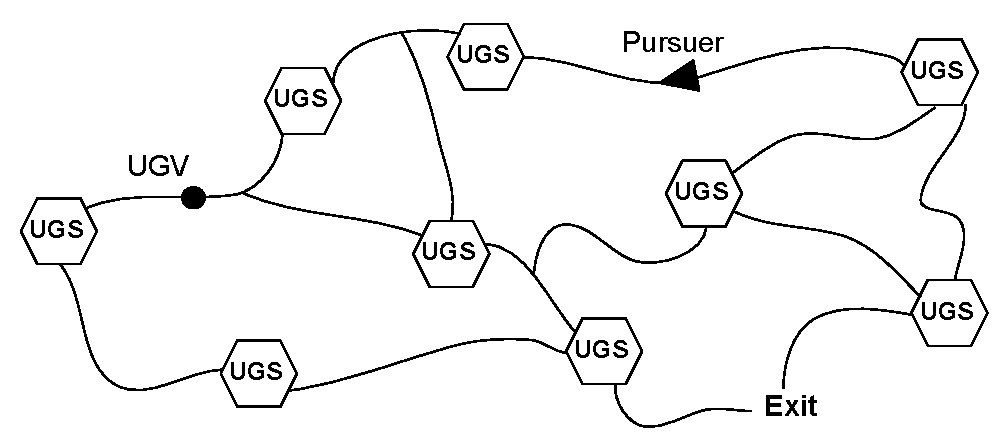
\includegraphics[width=0.5\textwidth]{Figures/RoadNet}
    	\caption{Application example of unmanned ground vehicle (UGV) in a road network, trying to evade a pursuer, using information from unmanned ground sensors (UGSs), as well as information and decision making advice from a human operator.} %The operator's actions towards the UGV are trust-based.}
        \label{fig:RoadNet}
    \end{figure}

    In this scenario the trust-cycle terms can be defined as follows: \textit{Artificially Intelligent Agent:} the UGV, which must make decisions under uncertainty with little information (the pursuer is only observed sporadically and does not follow a known course); \textit{Trust:} The operator's willingness to rely on the UGV when the outcome of the mission is at stake, such as in a scenario where the UGV is carrying a VIP or some other valuable payload; \textit{Trust-Related Behaviors:} operator's behaviors that indicate trust (or lack thereof) in the UGV, including the information and commands they give to the UGV. This might take the form of approving/rejecting the UGV's decisions, or real-time communication and adjustments of the UGV's information based on what the operator receives from other intelligence sources; \textit{Assurances:} properties and/or behaviors of the UGV that have an effect on the operator's trust. These can include communicating the probability of success for a given policy, or communicating that the mission is not proceeding as expected.

\subsection{Related Work}\label{sec:rel_work}
    The issues of interpretability, explainability, and transparency of AI has garnered considerable recent attention \cite{Doshi-Velez2017-xy, Weller2017-zx, Lipton2016-ug, Gunning2017-ih}. The related body of work has many interesting and important insights regarding the need for transparency, but does not formally acknowledge the role of trust in human decision making, or how interpretability and transparency affect the trust of those who use AIAs. Yet, this work is beneficial because it draws the attention of researchers to this critical area, and it initially formalizes the problem for those actively researching assurance design.

    \citet{Lillard2016-yg} addressed the role of assurances in the relationship between humans and AIAs, and provides much of the foundation used here for describing the relationships between assurances and trust in human-AIA interaction. Here, the framework for analyzing assurances is presented in a way that is both more general and more detailed, albeit with the same end goal of being applied in a very similar end application. For instance, we consider the full trust model presented by \citet{McKnight2001-fa}, whereas \citeauthor{Lillard2016-yg} only consider a subset of the trust model.

    Relating to the work of \citet{McKnight2001-fa}, who constructed a typology of interpersonal trust, we adopt the position that (besides being applicable to the e-commerce industry as originally intended) their trust model also applies to relationships between humans and AIAs (as in \cite{Lillard2016-yg}). They refer to something called `vendor interventions' that are related to assurances in this paper. One small, but important distinction from vendor interventions is that assurances cannot directly have an affect on the user trust-related behaviors (TRBs). This is an important point, since we are considering scenarios in which the human and AIA are working together, and not ones where the human is strictly dependent or steered/guided by an AIA. 
    
    While assurances are defined by \citeauthor{Lillard2016-yg}, and mentioned by \citeauthor{McKnight2001-fa}, and also \citeauthor{Corritore2003-gx}, we investigate in detail how assurances fit within the trust cycle (from Figure~\ref{fig:SimpleTrust_one_way}), survey what methods of assurance have been and are currently being used, then present a refined definition and classification of assurances. In essence, whereas others have noted the \textit{existence} of assurances, we now directly consider the question: What, exactly, \textit{are} assurances, and how can they be \textit{designed}? To that end we survey literature that formally considers trust between humans and AIAs, as well as literature that informally investigates trust through topics like transparency, explainability, and interpretability, and begin to distill ideas for practically designing assurances in human-AIA trust relationships. \brettcomm{I DON'T THINK THERE'S MUCH DISCUSSION OF THIS ANYWHERE\ldots}
